% Options for packages loaded elsewhere
\PassOptionsToPackage{unicode}{hyperref}
\PassOptionsToPackage{hyphens}{url}
%
\documentclass[
  ignorenonframetext,
]{beamer}
\usepackage{pgfpages}
\setbeamertemplate{caption}[numbered]
\setbeamertemplate{caption label separator}{: }
\setbeamercolor{caption name}{fg=normal text.fg}
\beamertemplatenavigationsymbolsempty
% Prevent slide breaks in the middle of a paragraph
\widowpenalties 1 10000
\raggedbottom
\setbeamertemplate{part page}{
  \centering
  \begin{beamercolorbox}[sep=16pt,center]{part title}
    \usebeamerfont{part title}\insertpart\par
  \end{beamercolorbox}
}
\setbeamertemplate{section page}{
  \centering
  \begin{beamercolorbox}[sep=12pt,center]{part title}
    \usebeamerfont{section title}\insertsection\par
  \end{beamercolorbox}
}
\setbeamertemplate{subsection page}{
  \centering
  \begin{beamercolorbox}[sep=8pt,center]{part title}
    \usebeamerfont{subsection title}\insertsubsection\par
  \end{beamercolorbox}
}
\AtBeginPart{
  \frame{\partpage}
}
\AtBeginSection{
  \ifbibliography
  \else
    \frame{\sectionpage}
  \fi
}
\AtBeginSubsection{
  \frame{\subsectionpage}
}
\usepackage{lmodern}
\usepackage{amssymb,amsmath}
\usepackage{ifxetex,ifluatex}
\ifnum 0\ifxetex 1\fi\ifluatex 1\fi=0 % if pdftex
  \usepackage[T1]{fontenc}
  \usepackage[utf8]{inputenc}
  \usepackage{textcomp} % provide euro and other symbols
\else % if luatex or xetex
  \usepackage{unicode-math}
  \defaultfontfeatures{Scale=MatchLowercase}
  \defaultfontfeatures[\rmfamily]{Ligatures=TeX,Scale=1}
\fi
% Use upquote if available, for straight quotes in verbatim environments
\IfFileExists{upquote.sty}{\usepackage{upquote}}{}
\IfFileExists{microtype.sty}{% use microtype if available
  \usepackage[]{microtype}
  \UseMicrotypeSet[protrusion]{basicmath} % disable protrusion for tt fonts
}{}
\makeatletter
\@ifundefined{KOMAClassName}{% if non-KOMA class
  \IfFileExists{parskip.sty}{%
    \usepackage{parskip}
  }{% else
    \setlength{\parindent}{0pt}
    \setlength{\parskip}{6pt plus 2pt minus 1pt}}
}{% if KOMA class
  \KOMAoptions{parskip=half}}
\makeatother
\usepackage{xcolor}
\IfFileExists{xurl.sty}{\usepackage{xurl}}{} % add URL line breaks if available
\IfFileExists{bookmark.sty}{\usepackage{bookmark}}{\usepackage{hyperref}}
\hypersetup{
  pdftitle={Final Presentation},
  pdfauthor={Collin Brehmer, Molly Hischke, Kyle Hancock, Nikki Johnson},
  hidelinks,
  pdfcreator={LaTeX via pandoc}}
\urlstyle{same} % disable monospaced font for URLs
\newif\ifbibliography
\usepackage{graphicx,grffile}
\makeatletter
\def\maxwidth{\ifdim\Gin@nat@width>\linewidth\linewidth\else\Gin@nat@width\fi}
\def\maxheight{\ifdim\Gin@nat@height>\textheight\textheight\else\Gin@nat@height\fi}
\makeatother
% Scale images if necessary, so that they will not overflow the page
% margins by default, and it is still possible to overwrite the defaults
% using explicit options in \includegraphics[width, height, ...]{}
\setkeys{Gin}{width=\maxwidth,height=\maxheight,keepaspectratio}
% Set default figure placement to htbp
\makeatletter
\def\fps@figure{htbp}
\makeatother
\setlength{\emergencystretch}{3em} % prevent overfull lines
\providecommand{\tightlist}{%
  \setlength{\itemsep}{0pt}\setlength{\parskip}{0pt}}
\setcounter{secnumdepth}{-\maxdimen} % remove section numbering

\title{Final Presentation}
\author{Collin Brehmer, Molly Hischke, Kyle Hancock, Nikki Johnson}
\date{12/13/2019}

\begin{document}
\frame{\titlepage}

\begin{frame}{Research Question}
\protect\hypertarget{research-question}{}

What positions on the Jeopardy board are most likely to be a Daily
Double?

\end{frame}

\begin{frame}{Introduction}
\protect\hypertarget{introduction}{}

\begin{itemize}
\tightlist
\item
  Importance to the game (James Holzhauer)
\item
  Other research
\item
  Challenge of finding position
\item
  Visual representation
\end{itemize}

\end{frame}

\begin{frame}{Methods}
\protect\hypertarget{methods}{}

\begin{itemize}
\tightlist
\item
  Only included episodes from dates beyond November 26, 2001
\item
  Finding x position of daily double (filtered to episodes with 12
  categories)
\item
  Finding y position of daily double (Weighted across missing values)
\end{itemize}

\end{frame}

\begin{frame}{Methods}
\protect\hypertarget{methods-1}{}

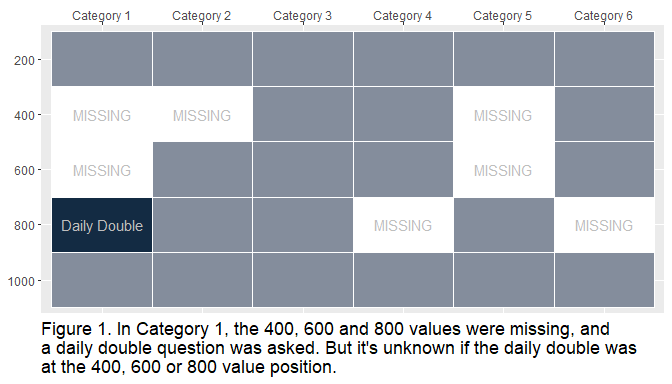
\includegraphics{final_presentation_files/figure-beamer/unnamed-chunk-2-1.pdf}

\end{frame}

\begin{frame}{Methods}
\protect\hypertarget{methods-2}{}

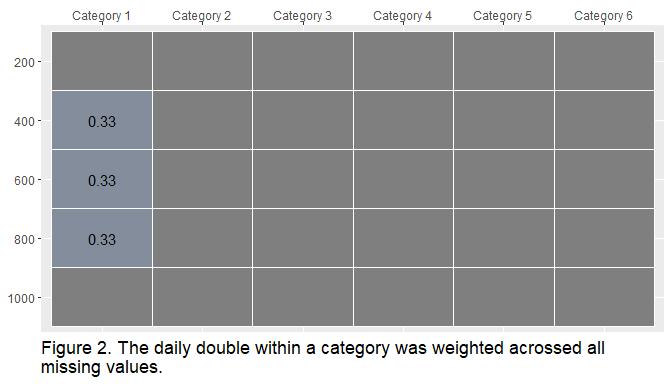
\includegraphics{final_presentation_files/figure-beamer/unnamed-chunk-3-1.pdf}

\end{frame}

\begin{frame}{Results}
\protect\hypertarget{results}{}

Flex Dashboard:

\begin{itemize}
\item
  Daily Double Round 1 since 2001
\item
  Daily Double Round 2 since 2001
\item
  Daily Double Location by year
\item
  Daily Doubles are not evenly distributed across the board
\item
  No differences in daily double location between Round 1 and Round 2
\item
  15 out of 19 years had daily doubles within the 800/1600 row
\item
\end{itemize}

\end{frame}

\begin{frame}{Conclusions}
\protect\hypertarget{conclusions}{}

\end{frame}

\begin{frame}{Overview of Approach}
\protect\hypertarget{overview-of-approach}{}

\end{frame}

\begin{frame}[fragile]{Interesting Packages or Techniques}
\protect\hypertarget{interesting-packages-or-techniques}{}

\begin{itemize}
\tightlist
\item
  \texttt{map()}, \texttt{mutate()}, and \texttt{join}
\item
  \texttt{plot\_ly()}
\end{itemize}

\end{frame}

\begin{frame}{Lessons Learned}
\protect\hypertarget{lessons-learned}{}

\end{frame}

\end{document}
